\section{Neural network implementation and models}
Building neural network for classification of pain maps was trial and error process.
In this project, the deep learning method is used to classify the pain maps and gender according to determined outputs. The data is a set of 2D-images combined with gender and the outputs are pain intensity and duration. For classification purpose, the supervised convolutional neural network is used followed by fully-connected layers at the end. This architecture of the model is chosen to the interest of morphology and location of the pain. The models are trained, and tested on a single computer with GPU and ran on Python programming language with Keras library. Specifications of hardware and software are described in detail in \autoref{sec:softHard}.

\subsection{Software and hardware}\label{sec:softHard}
The neural networks developed for this study was programmed using Python v3.6.3. Python is an object-oriented and general-purpose programming and scripting language, that may be used for e.g. programming websites, mobile applications, but also for machine learning programming applications.
For the development of deep learning application in python, different libraries are available, where some of the popular is the Theano and TensorFlow libraries \citep{Swamynathan2017}. The Tensorflow v1.3.0 library was chosen for this study. %TensorFlow is an open source library for development of machine learning applications, that has been released by Google \citep{Swamynathan2017}. 
An additional library, Keras v2.0.8, was imported, which runs on top of either Tensorflow or Theano and is a high-level neural networks application programming interface (API).  
Keras is a simplified version of the two libraries, which allows for fast and easier prototyping of neural network \citep{Chollet2015}. This was deemed suitable given that no previous experience with the neural network was available during this study. 
\noindent
Utilization of graphics processing unit (GPU) computation was also implemented using CUDA drivers and cnDNN communication libraries, which allowed for faster runtimes, then through the use of the central processing unit (CPU).
%Keras is a simplified version of the two libraries, which makes it easier to program in Python, but still allows for building complex models. TensorFlow is an open source library for development of machine learning applications, that has been released by Google \citep{Swamynathan2017}.
%Using CPU or GPU on this platform the most mathematical operation is computed in a computerized and simple way \citep{Swamynathan2017}. A small example of the concept of using TensorFlow could be seen in Appendix B. The plots for this model are generated using Tensorboard visualizing tool. It allows to watch a graph during the training, gives plot quantitative metrics and shows data like images that pass through it. Besides visualizing part of this tool it is also useful for debugging as it allows to observe the graph at a present time.\citep{Abadi2016a}

\noindent
The neural network was developed on a laptop with 4x 'Intel® Core™ i7' CPU‘s and one GPU type 'Geforce GTX 970M' with specifications listed in table \ref{tab:Specs}.

%\begin{figure} [H]
%\centering
%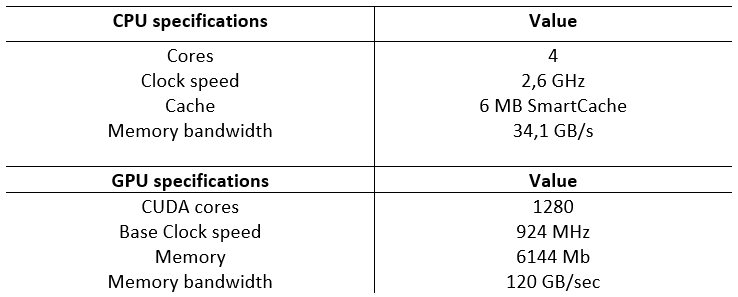
\includegraphics[width=1\textwidth]{figures/Specs}
%\caption{Specifications of CPU‘s and GPU \citep{Intel,Nvidia}.}
%\label{tab:Specs}
%\end{figure}

\begin{table}[H]
\centering
\begin{tabular}{p{4cm}|p{4cm}}
\hline
CPU specifications &  Value \\ \hline
Cores & 4 \\
Clock speed & 2.6 GHz \\
Cache & 6 MB SmartCache  \\
Memory bandwidth & 34.1 GB/s \\ \hline
GPU specification & Value \\ \hline
CUDA cores & 1280  \\
Base Clock speed & 924 MHz  \\
Memory & 6144 MB  \\
Memory bandwidth & 120 GB/s  \\ \hline
\end{tabular}
\caption{Specifications of CPU and GPU \citep{Intel,Nvidia}}
\label{tab:Specs}
\end{table}

\subsection{Design choices and model architecture}
This section presents the different models, their architecture, and implementation used in this study.
For classification of each pain map representation, a corresponding model was made. The classifier models for morphology- and combined-representation were operating on a pixel level by learning features of the pain charts, whilst the location-representation operated from the 10 element location vector.
The architecture of the models consists of two main parts, a convolution part, and a fully connected part, except the location model that only consist of the latter.  
Convolution works as feature extraction of the pain maps, where convolutional and pooling layers alternate in order to extract relevant features from the image, as described in section \autoref{sec:Layers}.
The fully connected part works as classification, where computed feature maps get weighted and classified to a particular class in the output layer.
A higher generalization performance of the classifiers was investigated through the use of regulation and optimization methods.
The available data was separated into a training and test subsets, from which training data was used to regulate and optimize the model.
Supervised learning was used for training the models. The common input for all of the models was gender, along with the different pain map representations.

%, as presented in figure \ref{fig:schema1}.
% These inputs are trained and then compared against their respective category label.

%From the higher point of view, the model can be architecturally split into two main parts. Feature extraction part, where convolutional and pooling layers alternates in order to extract the most important features out of the image. Second part is called classification, where computed feature maps will be assigned to particular class of the output layer. In order to obtain a higher generalization performance of deep learning classifier, methods like activation function, regulation and optimization will be used within the layers were implemented into the models.


\subsubsection{Morphology-representation models}
The models for the morphology-representation consists of convolution, max pooling, and fully connected layers. 
The models are essentially made up of two parts, where one is the extraction of image features, and another being a classification part.
For the extraction of image features a series of three convolutional and max-pooling layer are stacked after each other, to which the first layer is specified to receive the main input of the shape $1 \times 118 \times 252$ where 1 reflects the fact that the pain map representation is binary.
The classification part of the network is the same architecture as that of the model for the location-representation and thereby consists of fully connected layers. Between these two parts of the model, a secondary input is added specifying the gender related to the given pain map.
Before the pain maps, features reach the fully connected layers it is flattened from the shape of a matrix to that of a single row in order to merge the extracted features with gender. The merged data passes through fully connected layers and reaches the output layer where it is given a percentage value according to which class it fits the most.
The architecture of the morphology representation model is shown in figure \ref{fig:Schema1}.

\begin{figure} [H]
\centering
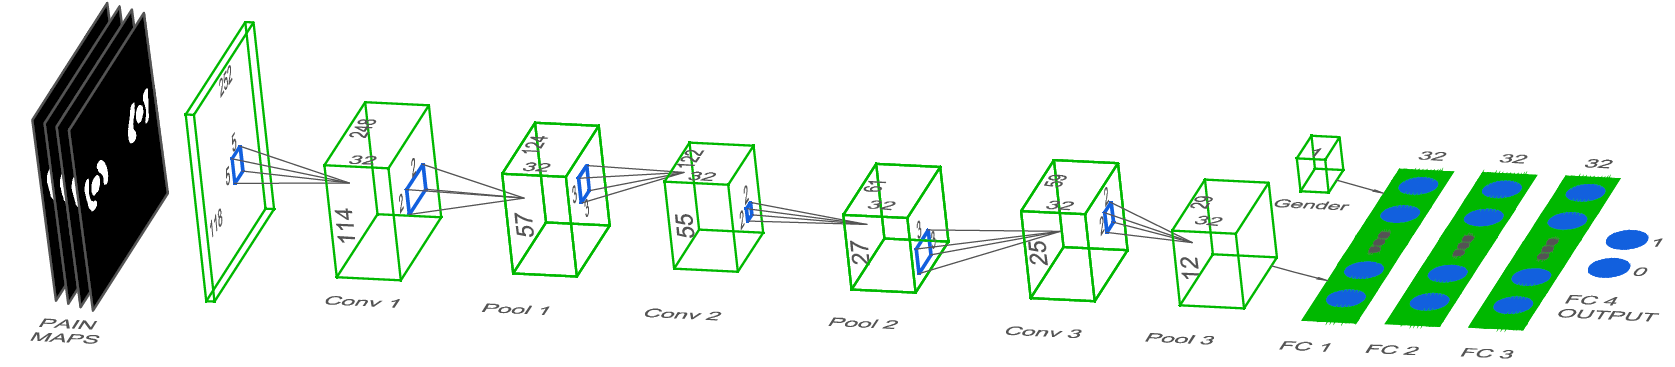
\includegraphics[width=1.0\textwidth]{figures/models}
\caption{Architecture of the neural network models.}
\label{fig:Schema1}
\end{figure}


\subsubsection{Location-representation models}
Given the location-representations a simplicity, in the form of an 11 element row-vector that contains both the pain maps information along with a gender value as described in section \ref{sec:Regions}, the architecture of the model is also relatively simple, compared to the other models. 
For this representation, the model consists of four fully-connected layers where the last of the layers is the output layer, where the number of outputs matches the number of classes.
It was chosen not to use convolution layers, like in the morphology- and combined-representation, because it was believed that there would be no greater benefit given how convolution works, and the size of the location-representation.
An overview of the architecture of the model for the location-representation can be seen in figure \ref{fig:locationar}.

\begin{figure} [H]
\centering
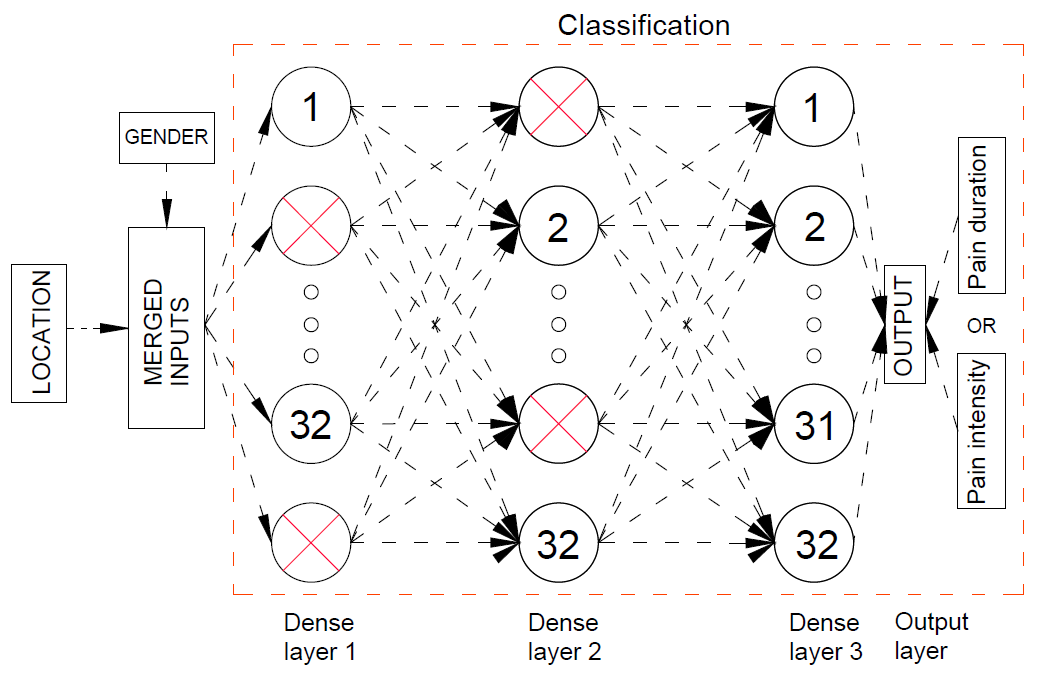
\includegraphics[width=0.8\textwidth]{figures/locationar}
\caption{Architecture of the location-representation model.}
\label{fig:locationar}
\end{figure}

\subsubsection{Combined-representation models}
The architecture of this model is nearly identical to that of the morphology-representation model, as seen in figure \ref{fig:Schema1}.
The main difference can only be seen in the dimension of input for the pain map representation, where the input shape is $10 \times 118 \times 252$ to which 10 is the number of image layers per pain map. This is the result of the one-hot encoding done to the images as described in section \ref{sec:combined}.


\subsection{Data handling in python}
Pre-processed data is loaded from a \textit{.mat} file into Python.
Data within the file was pre-shuffled to ensure that the pain maps separated into a training, validation and test subsets randomly. The different subsets were respectively made up of 75\%, 10\% and 15\% of the available pain maps. The data was separated to clearly distinguish between dataset and their purpose, and thereby prevent the same data from being used for training and e.g testing since this would give a wrong estimation of the model’s performance.
The training and validation subsets were used to train and optimize the models, to find the optimal weights with the back-propagation algorithm \citep{Bengio2012}.
The test subset was for final testing of the model, to get an estimation of the ability to generalize "unseen" pain maps.
Additionally, the models for the morphology- and combined-representation, the data was reshaped from a row vector, back into a matrix to retain their 2D structure of the pain map.
The true classification labels were one-hot encoded to make the number of classes compatible according to the number of outputs in the output layer.

\section{Optimization-process of the models}
To reduce overfitting and improve general performance of the model, different methods were implemented and test.
A grid search method was used to find initial hyperparameters for the models. For this method, a set of different hyperparameters were defined and tested using a 10-fold cross-validation, where the hyperparameters that resulted in the highest accuracy were chosen, and can be seen in appendix \ref{app:opti}. Learning rate, type of initializer, number of nodes, batch size and number of epochs were tested using this method. 
An additional manual optimization was then performed, where all the changes to the hyperparameters were based on the behavior of the validation set during training of the deep learning models.
The development of the learning process was visually evaluated by plotting the accuracy and loss of both the training and validation subset. According to number of the epoch when the models start to overfit, changes to learning rate, epochs, batch size, momentum, and a number of nodes were made if needed. The examples of the accuracy, loss plots, and overfitting could be seen in Fig. \ref{fig:Graphs}.

\begin{figure} [H]
\centering
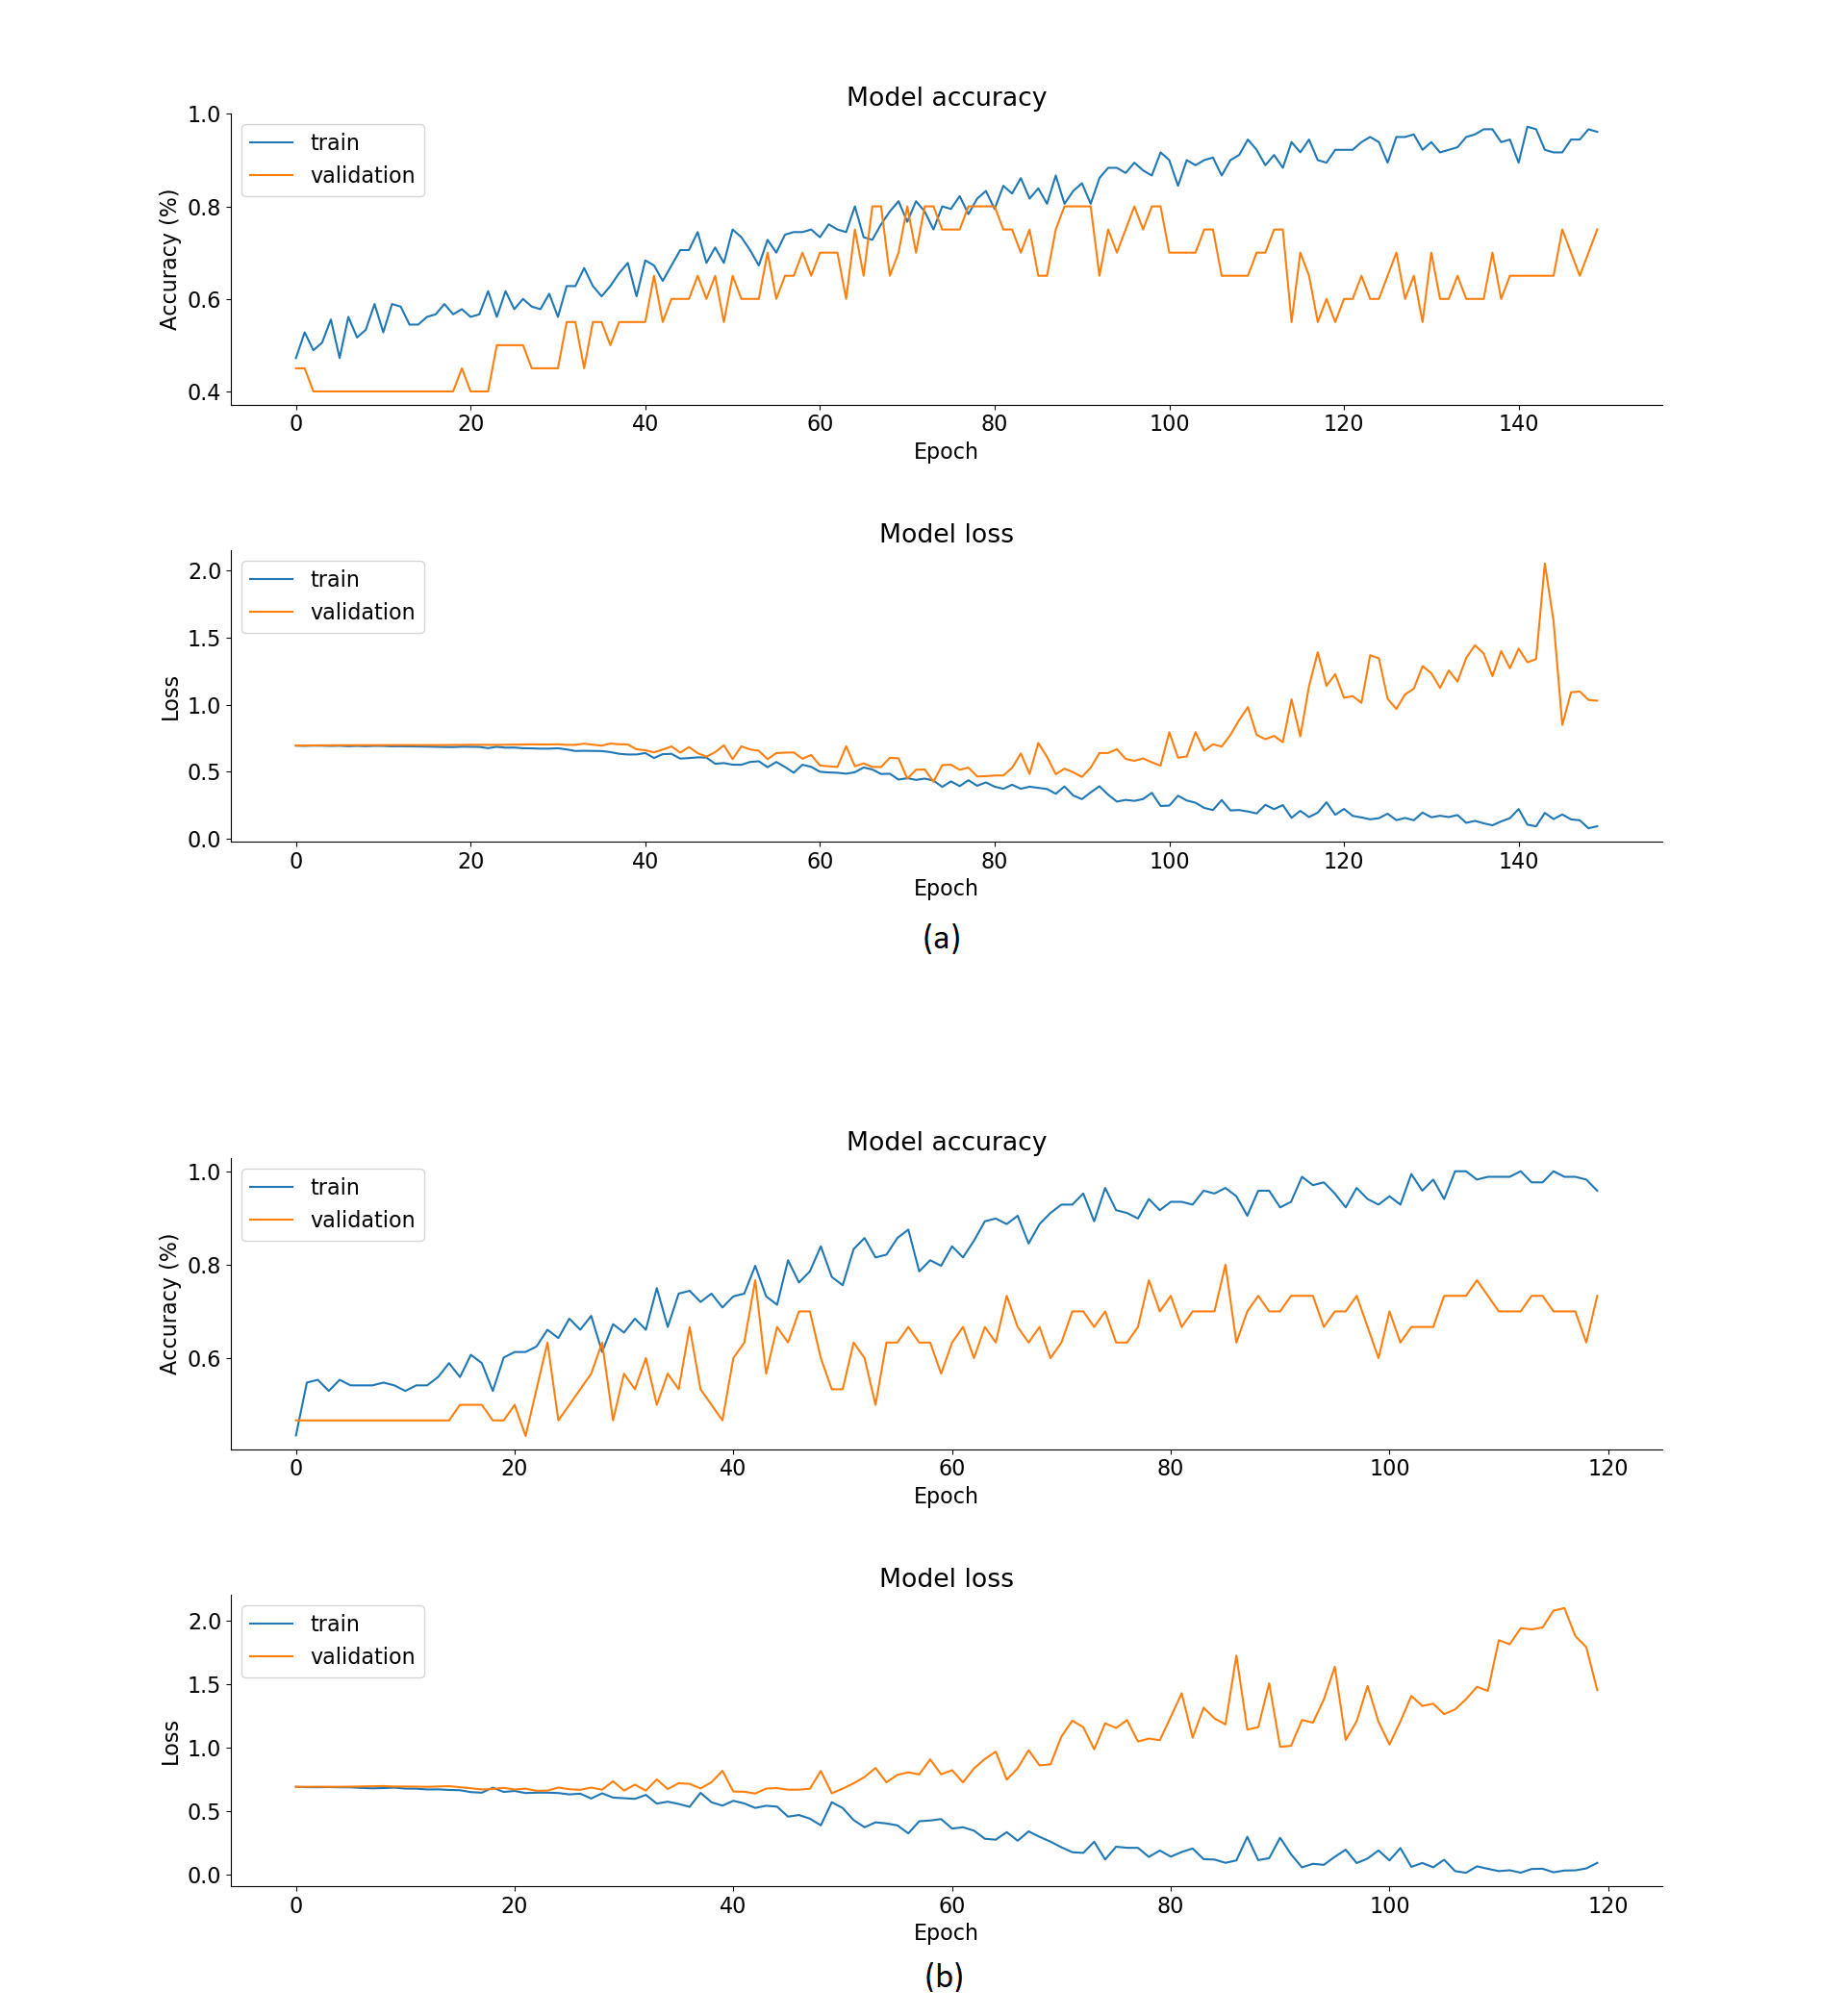
\includegraphics[width=0.8\textwidth]{figures/Graphs}
\caption{Graphs of the models accuracy, loss, and overfitting on training and validation datasets: (a) model of combined-representation according to the duration, (b) model of the morphology-representation according to the duration}
\label{fig:Graphs}
\end{figure}


\subsubsection{Activation function}
For all models the activation function in all layers except the output layer was the ReLU function. This was chosen as this is seen as the most common activation function in more modern neural networks. The reason for its popularity is that it prevents the problem known as the vanishing or exploding gradient, typically seen when using sigmoid activation function in the hidden layers.\citep{Goodfellow2016}   
All output layer activation functions were chosen as sigmoid, because it was stated as the typical activation function for output classification problem \citep{Duda2000}.

\subsubsection{Dropout}
Dropout was implemented in the models due to the benefits described in section \ref{sec:dropout}, where it is written that dropout should be used to reduce overfitting of the models. A dropout was then implemented within the hidden fully connected layers of all models, except the output layer, and set to randomly drop 50\% of the nodes. 


